\documentclass{standalone}
\usepackage{pgfplots}
\pgfplotsset{compat=newest}
\usepgfplotslibrary{patchplots}
\begin{document}
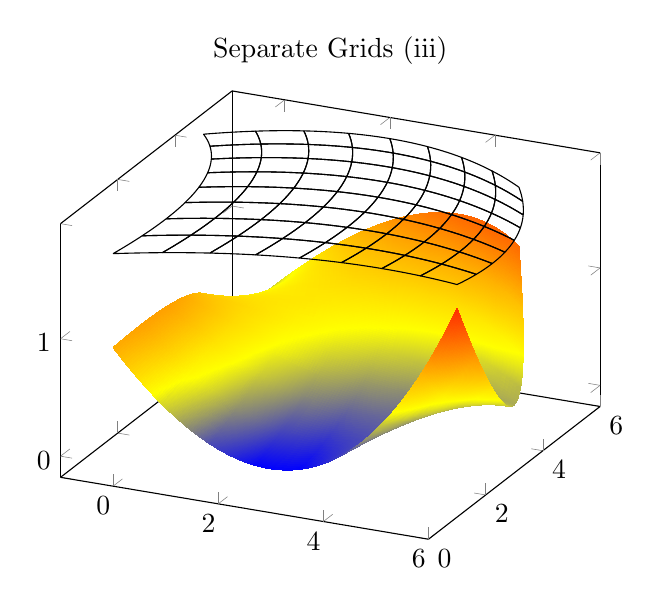
\begin{tikzpicture}
\begin{axis}[
	title={Separate Grids (iii)}]
\addplot3[patch,patch type=biquadratic,shader=interp,
	patch refines=3]
coordinates {
	(0,0,1) (6,1,1.6) (5,5,1.3) (-1,5,0)
	(3,1,0) (6,3,0.4) (2,6,1.1) (0,3,0.9)
	(3,3.75,0.5)
};
\addplot3[patch,patch type=biquadratic,
	mesh,black,
	z filter/.code={\def\pgfmathresult{1.8}},
	patch refines=3]
coordinates {
	(0,0,1) (6,1,1.6) (5,5,1.3) (-1,5,0)
	(3,1,0) (6,3,0.4) (2,6,1.1) (0,3,0.9)
	(3,3.75,0.5)
};
\end{axis}
\end{tikzpicture}
\end{document}
